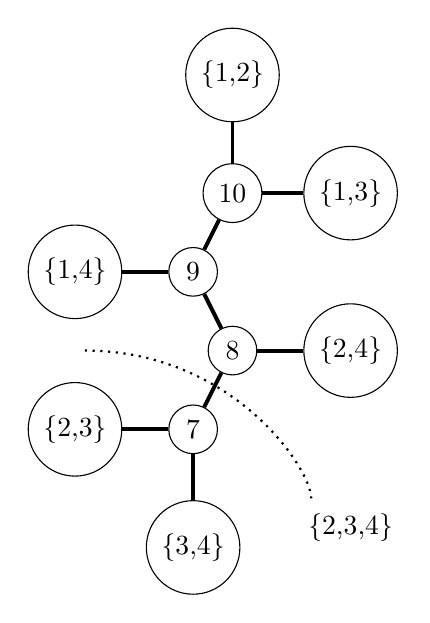
\begin{tikzpicture}
	\begin{scope}[xshift=6cm, yshift=0cm]
		\node[circle, draw, color=black, fill=white] (b1) at (3, 4) {\{1,3\}};
		\node[circle, draw, color=black, fill=white] (b3) at (-0.5, 3) {\{1,4\}};
		\node[circle, draw, color=black, fill=white] (10) at (1.5, 4) {10};
		\node[circle, draw, color=black, fill=white] (9) at (1, 3) {9};
		\node[circle, draw, color=black, fill=white] (8) at (1.5, 2) {8};
		\node[circle, draw, color=black, fill=white] (7) at (1, 1) {7};
		\node[circle, draw, color=black, fill=white] (b2) at (3, 2) {\{2,4\}};
		\node[circle, draw, color=black, fill=white] (b4) at (-0.5, 1) {\{2,3\}};
		\node[circle, draw, color=black, fill=white] (b5) at (1, -0.5) {\{3,4\}};
		\node[circle, draw, color=black, fill=white] (b6) at (1.5, 5.5) {\{1,2\}};
	
		% Draw the edges between nodes with labels
		\draw[line width=0.5mm, color=black] (10) -- (b6);
		\draw[line width=0.5mm, color=black] (b1) -- (10);
		\draw[line width=0.5mm, color=black] (b3) -- (9);
		\draw[line width=0.5mm, color=black] (10) -- (9);
		\draw[line width=0.5mm, color=black] (9) -- (8);
		\draw[line width=0.5mm, color=black] (b2) -- (8);
		\draw[line width=0.5mm, color=black] (8) -- (7);
		\draw[line width=0.5mm, color=black] (7) -- (b4);
		\draw[line width=0.5mm, color=black] (7) -- (b5);

		\node (G) at (3, -0.25) {\{2,3,4\}};

		\node[opacity=0] at (-0.5, 2) (start) {};
		\node[opacity=0] at (2.5, 0) (end) {};
		\draw[dotted, thick] (start) .. controls +(2,0) and +(0,0.5) .. (end);
	\end{scope}
\end{tikzpicture}
